\section{Propri�t�s �l�mentaires}

Ceci constitue d�j� une grande cat�gorie d'espaces r�flexifs. Il serait int�ressant � ce stade de savoir s'il existe une certaine stabilit� dans la classe des espace r�flexifs, et si oui, de quelle nature. C'est ce � quoi on va s'affairer dans cette section.

\begin{Def}
Soient $E$ et $F$ deux espaces vectoriels norm�s, et $T:E\maps F$ une application lin�aire continue. L'ajointe de $T$ est not�e $\adj{T}$ et d�finie par

\[
\begin{array}{lllll}
\adj{T}&:&F\dual&\maps&E\dual\\
&:&y\dual&\mapsto&y\dual\circ T
\end{array}
\]
\end{Def}

De plus, c'est une application lin�aire continue et $\norme{\adj{T}}=\norme{T}$.

\begin{Prop}\label{isoreflex}
Soit $T:E\maps F$ un isomorphisme d'espaces vectoriels norm�s. Alors

\begin{enumerate}[(1)]
\item L'application $\adj{T}$ est un isomorphisme
\item Si $E$ est r�flexif, alors $F$ aussi
\end{enumerate}
\end{Prop}
\begin{proof}
~

(1)\\
%
Puisque $\adj{T}$ est continue, il suffit de montrer que c'est une bijection et le th�or�me des isomorphismes de Banach nous donnera la continuit� de l'inverse.

$\adj{T}$ est injective:\\
%
Soit $y\dual\in F\dual$ tel que $\adj{T}(y\dual)=0$. On a que $y\dual(T(x))=0$ quelque soit $x\in E$. Puisque $T$ est bijective, c'est �quivalent � dire que $y\dual(y)=0$ quelque soit $y\in F$, c'est-�-dire que $y\dual=0$.\newline

$\adj{T}$ est surjective:

Soit $x\dual\in E\dual$. On prend $y\dual=x\dual\circ\inv{T}\in F\dual$. Soit $x\in E$, alors

\[
\adj{T}(y\dual)(x)
=
y\dual(T(x))
=
x\dual(\inv{T}(T(x)))
=
x\dual(x)
\]

D'o� $x\dual=\adj{T}(y\dual)$.\newline

(2)\\
%
Soit $y\bidual\in F\bidual$. Puisque $T$ est un isomorphisme, on sait par (1) que $\biadj{T}$ est �galement un isomorphisme. De plus, $E$ est r�flexif, par cons�quent il existe $x\in E$ tel que $\biadj{T}(ev_x) = y\bidual$. Soit $y\dual\in F\dual$. On a

\[
y\bidual(y\dual)
=
ev_x(\adj{T}(y\dual))
=
(\adj{T}(y\dual))(x)
=
y\dual(T(x))
=
ev_{T(x)}(y\dual)
\]

D'o� $y\bidual=ev_{T(x)}$, donc $F$ est r�flexif.
%\raisebox{-0.6\height}{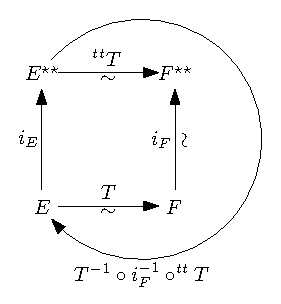
\includegraphics[scale=1]{rappels/diagrammeisodual.eps}}
\end{proof}


